


Clip, short for the Cologne Laue Indexation Program, is a software for
the analysis of Laue images. It is provides a semi-automatically
indexing function, the possibility to further refine a solution and
allows to calculate the required rotations to reorient the crystal. It
supports multiple crystals and projections at the same time. A unique
feature is the native support for the 12-bit gray scale images of the
Fuji BAS image plate scanner, which is used at the institute Laue
camera. Here it has been used very successful since 2006.

The software is written in the Python language \cite{pythonRM} for a
reduced development time. Most code was first implemented in Python
and only speed critical parts were rewritten in C++ and exposed to
Python with the SIP interface generator \cite{SIP_River}. The
graphical user interface is realized with the help of the Qt
\cite{Qt4} toolkit and it's python bindings PyQt \cite{PyQt4}. The use
of the cross-platform toolkit Qt and Python allows the use on Linux,
Windows and Max OS X computers. For the Windows platform, a stripped
down install package including an embedded version of the python
interpreter is available.  This withdraws the need for a full python
installation including PyQt, numpy, scipy and the python image
library. The program is licensed under the terms of the Gnu General
Public License \cite{GPL} and is publicly available at
\url{http://clip.berlios.de}.


\section{The Program}


\subsection{Main Window}

\begin{figure}[htb]
\center{
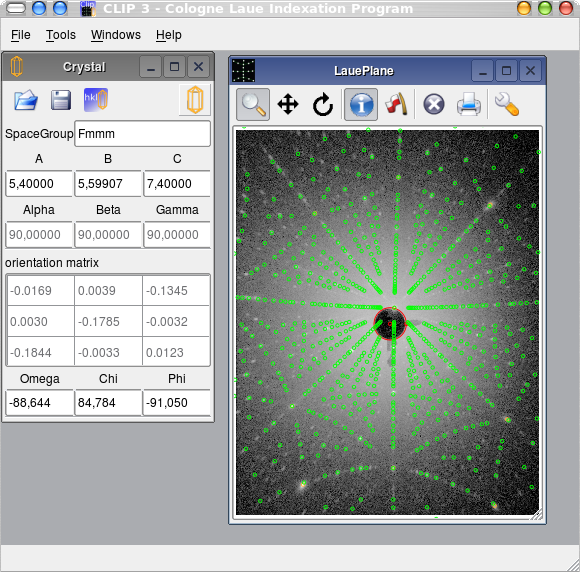
\includegraphics[width=0.65\textwidth]{clip/Clip_main}
} \label{Clip:FigMainWindow}
\caption[Main window of Clip]{Clip main window with crystal definition
  and a Laue Plane}
\end{figure}

Figure \ref{Clip:FigMainWindow} shows the main window of Clip with the two
principal sub-windows, the crystal definition and the Laue
projection plane.

The work paradigm is to define one or several crystals and connect it
to projectors, which then display a pattern according to their type.
One crystal could be connected to possibly many projectors, while a
projector is only connected to a single crystal. The majority of cases
will only employ a single crystal and a single projector. As said
before, the projector determines the type of projection. Up to know, a
stereographic projection of reciprocal lattice vectors and a planar
projection of the emergent wave vector (the Laue photograph on a flat
film) are Implemented. But other types of projectors could be written,
like a projection on a cylindrical detector or a gnomonic projection.

The Crystal and projector windows could be played from the File Menu.
Additionally, the complete workspace could be saved and restored. The
Workspace includes all crystals and the projectors connected to
them. The window layout and all relevant data are saved to a
xml-file. This allows to save the result of an indexing, including
the refined parameters and the marked spots.

The Tools menu contains the tool windows, which are described below in
their occurrence in a typical workflow.


\subsection{Crystal Window}


\begin{figure}[htb]
\centering
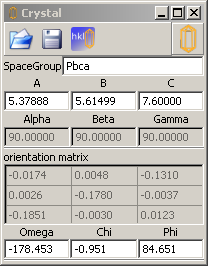
\includegraphics[width=0.35\textwidth]{clip/Tool_Crystal}
\label{Clip:FigToolCrystal}
\caption{Crystal parameter input window.}
\end{figure}

Figure \ref{Clip:FigToolCrystal} shows the input box for the crystal
parameters. The three tool buttons allow th save and load the crystal
definition to a xml file and to start the indexing procedure
respectively. The xml-file contains the space group, the lattice
parameters and the three Euler angles. The crystal icon in the upper
right corner could be dragged to a projection window to connect them.

Below, one finds the inputs for the space group and the lattice
constants. The space group determines the free lattice parameters
(e.g. all angle parameters are fixed to 90$^\circ$ for the
orthorhombic space groups) and which equivalent solutions in the
indexing procedure should be suppressed. The program uses a very
relaxed checking of the space group . Everything which is formally correct
should be accepted, e.g. F1, F4/mmm, Pbaa but not Paaa. At the moment
systematic extinctions, even for the lattice centering, are not
handled, therefore e.g. Pmmm, Pnma and Fmmm would give exactly the
same result.  not handled by the program A special behavior is
implemented for the trigonal space groups. If entered as e.g. R3m, the
program uses the rhombohedral primitive setting a=b=c,
$\alpha=\beta=\gamma$, when entered using the non-standard centering
symbol ``H'' (H3m) the hexagonal setting a=b$\ne$c,
$\alpha=\beta=90^\circ, \gamma=120^\circ$ is used. When changing
directly between these space-group symbols, the lattice constants are
converted accordingly and a rotation is employed in order to get an
equivalent projection. This rotation ensures, that the
\hkl[111]$_{rhom}$ and \hkl[1 -1 0]$_{rhom}$ coincides with the
\hkl[001]$_{hex}$ and \hkl[100]$_{hex}$ respectively after the
transformation.

Beneath the space group input, the inputs for the lattice constants
are located. Depending on the space group, some of the fields may be
disabled, for a cubic space group, only the a lattice constant is
available.

Underneath the lattice constants the orientation matrix and three
Eulerian angles follow. The orientation matrix displays the reciprocal
lattice vectors in a Cartesian laboratory system. The system employed
in the program maps the x-, y- and z-axis to the primary beam axis,
the horizontal and the vertical axis respectively. The Euler angles
$\Omega$, $\chi$ and $\Phi$ qualify the rotations around the z-, x-
and y-axis respectively. The initial orientations of the crystal,
e.g. with all Euler angles set to zero, places the crystallographic
\textbf{a}-axis on the x-axis, the \textbf{b}-axis in the xy-plane and
the \textbf{c}-axis completes the right handed system.


\subsection{Laue Plane}

The Laue plane window represents the film/image plate, where the Laue
pattern will be recorded on. It displays the recorded image, the
primary beam marker, marked reflexes and the calculated spots and
allows to zoom in to the image and mark reflexes.


\begin{figure}[htb]
  \centering
  \begin{minipage}[b]{0.4\textwidth}
    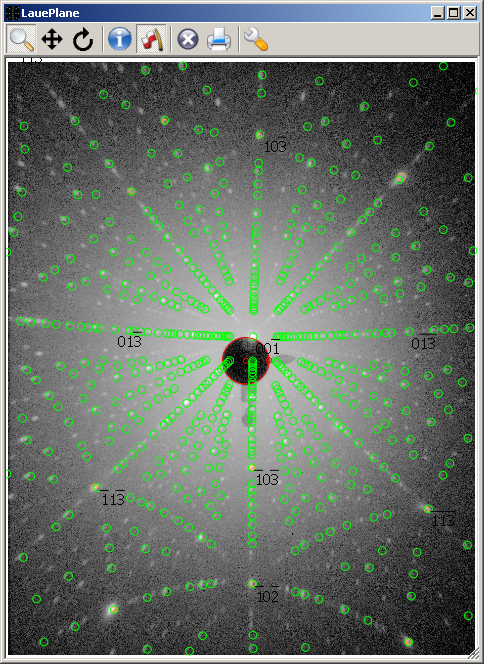
\includegraphics[width=\textwidth]{clip/Tool_LauePlane}
    \label{Clip:FigToolLauePlane}
    \caption[Laue plane window]{Laue plane window with a back reflection Laue image of
      SmTiO$_3$ from \cite{RothDiss}}
  \end{minipage}
  \imgspace{}
  \begin{minipage}[b]{0.4\textwidth}
    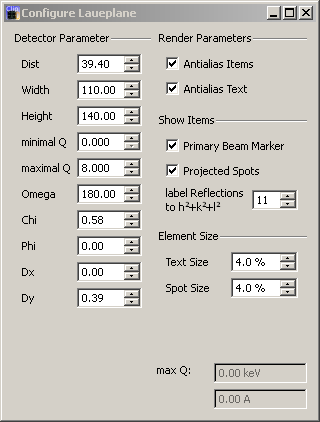
\includegraphics[width=\textwidth]{clip/Tool_CfgLauePlane}
    \label{Clip:FigToolCfgLauePlane}
    \caption[Laue plane configuration window]{Configuration panel for a Laue plane window.}
  \end{minipage}
\end{figure}



Two concentric red circles, the outer one with a handle, are the
primary beam marker. With the help of the handle, the outer circle could be
resized to increase the accuracy, if the Laue image provides an
appropriate feature, like the image plate system at does.

The mouse action depends on the selected button in the upper toolbar.

A left mouse button click and subsequent drag may either zoom into the
image or may rotate the crystal. Two rotation modes are available, the
first uses rotations around arbitrary axes in order to allow to freely
drag reflexes on the plane while the second rotates the crystal around
a fixed axis. This could be specified by the context menu or the
rotate window \ref{Clip:SecRotateWindow}

A simple left mouse click either creates a info panel for the nearest
reflex or adds a marker for indexing and fitting purposes. Info panels
and markers could be dragged around with the mouse. The info panels
will also be displayed on a print out and will disappear when the
crystal orientation is changed.

A short left click restores the previous zoom level and a
longer right mouse click opens a context menu. Here the rotation axis
could be set to reciprocal lattice vector of the nearest\footnote{to
  the actual mouse position} (calculated) reflex, all reflex informations
could be cleared and the nearest or all marked reflexes could be
cleared.

The three rightmost buttons on the toolbar allow to open or close a
Laue image, to print the Laue plane including all decorations and to
open the configuration dialog for this Laue plane. The image file may be
any image format known to the Python Image Library. Additionally the
program is able to read the format which is returned by the Fuji BAS
image plate reader. This format has a higher dynamic range of 12 bits,
compared to 8 bits of conventional gray scale image formats. In order to take
advantage of this improved range, the image is internally represented
with the full information and mapped to screen colors by a user
modifiable transfer curve, see \ref{Clip:SecTransferCurve}
If an image is loaded, four more buttons for image rotation and
flipping appear. 


Figure \ref{Clip:FigToolCfgLauePlane} shows the configuration
dialog. On the left are the parameters of the projection. From top to
the bottom they are:

\begin{description}
\item[Dist] Distance from the crystal to the projection plane.
\item[Width] Width of the projection plane. If a BAS image is read,
  this parameter is taken from the image.
\item[Height] Height of the projection plane. If a BAS image is read,
  this parameter is taken from the image.
\item[minimal Q] Lower bound of the wave vector distribution in
  \AA$^{-1}$. Could be normally set to 0.
\item[maximal Q] Upper bound of the wave vector distribution in
  \AA$^{-1}$. A higher value produces more spots and may slow down the
  program. The upper bound is also shown in the lower right corner as
  xray tube voltage\footnote{also corresponds to the electron energy}
  and x-ray wavelength.
\item[Omega, Chi] spherical coordinates of the plane normal. $\Omega$
  is the rotation around  the z-axis, therefore $\omega$=0$^\circ$
  corresponds to a transmission Laue configuration, while
  $\omega$=180$^\circ$ corresponds to a back reflection Laue
  configuration. $\chi$ is th polar angle.
\item[Phi] Rotation of the plane around the plane normal.
\item[Dx and Dy] Position of the piercing point of the plane and the
  plane normal, connecting the plane with the crystal.
\end{description}

On the right side, on finds parameters which alter the appearance of
the display. The render parameters allow to switch on or off the
anti-aliasing for the text and the items like projected reflex
markers. Anti-aliasing provides better quality but may be slower.

Next category allows to show or hide the primary beam marker and the
projected spots. The latter is very useful when one marks spots for
indexing. Additionally, one could specify, up to which value of
h$^2$+k$^2$+l$^2$ the hkl should be displayed beside the reflexes.
Contrary to the reflex info panels, these indicators move along with
the reflexes and allow a quick navigation in the reciprocal space.

Finally the Element Size category allows th specify the size for
the calculated spots and all text at the plane.


\subsection{Index Search}
\label{Clip:secIndexing}

\begin{figure}[htb]
  \centering
  \begin{minipage}[b]{0.45\textwidth}
    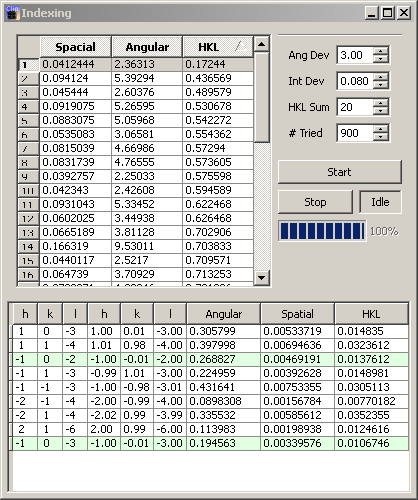
\includegraphics[width=\textwidth]{clip/Tool_Index}
    \label{Clip:FigToolIndex}
    \caption{Indexing tool window.}
  \end{minipage}
  \imgspace{}
  \begin{minipage}[b]{0.35\textwidth}
    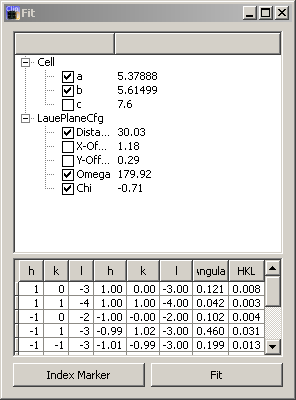
\includegraphics[width=\textwidth]{clip/Tool_Fit}
    \label{Clip:FigToolFit}
    \caption{Fit window}
  \end{minipage}
\end{figure}




Image \ref{Clip:FigToolFit} shows the indexing tool. In order to start
the indexing procedure, the correct space group and lattice constants
should be specified, the detector-sample distance should be correctly
entered in the configuration dialog\footnote{a distance of
  \unit[30]{mm} is default}, the primary beam marker should be moved
to the appropriate position and some likely low indexed spots should
have been marked\footnote{Choosing the suitable one depends very much
  on the experience of the experimenter}.  When the setup is complete,
one could start the indexing and hope, the correct solution is among
the calculated ones. Otherwise one should mark different spots and/or
try to modify the lattice constants and detector distance. If this
does not lead to the proposed result, ask an expert.


The algorithm used in the indexing procedure works as follows.  For
each marked spot, the direction \textbf{n}$_i$ of the scattering
vector is calculated. The magnitude is not accessible because of the
Laue geometry, so the n$_i$ are unit vectors. If k$_i$ denotes the
length of the scattering vector, then indexing the pattern stood for
determine a rotation matrix R and a set of integer vectors
\textbf{h}$_i$ so that

\begin{displaymath}
\textnormal{k}_i \cdot \mathbf{n}_i = \textnormal{R} \cdot \sum_j \mathbf{a}^*_j
\cdot \textnormal{h}_{i,j} = \textnormal{R} \cdot \Re \cdot \mathbf{h}_i
\end{displaymath}

is fulfilled with the reciprocal lattice vectors $\mathbf{a}^*_i$ and
the matrix of reciprocal basis vectors $\Re$.  This could be
transformed to

\begin{equation}
s_i \cdot \Re^{-1} \cdot \textnormal{R}^{-1} \cdot \mathbf{n}_i
= (\textnormal{h k l})
\label{Clip:eqnHKL}
\end{equation}

with appropriate scale factors $s_i$. In the actual procedure, the hkl
will only be almost integer.  To determine the rotation matrix R, a
set of reciprocal lattice vectors \textbf{t}$_i$ is created, sorted
according to h$^2$+k$^2$+l$^2$ and normalized. The first N vectors are
used as test vectors, the number is adjustable with the parameter
\textbf{\# Tried}.  Then for each pair of test vectors
(\textbf{t}$_i$, \textbf{t}$_j$) the angle between them is calculated
and compared to the angles between scattering vectors (\textbf{n}$_i$,
\textbf{n}$_j$). If pairs are found, whose angles differ by no more
than the parameter \textbf{Ang Dev}, an optimal rotation matrix R$_t$
is calculated, so that \textbf{t}$_i$ = R$_t^{-1}$ $\cdot$
\textbf{n}$_i$ and \textbf{t}$_j$ = R$_t^{-1}$ $\cdot$ \textbf{n}$_j$.

Know for the rest of the scattering vectors \textbf{n}$_i$, the vector
$\Re^{-1} \cdot \textnormal{R}^{-1} \cdot \mathbf{n}_i$ is calculated.
If the rotation matrix R$_t$ represents a feasible indexing, this
vector could be scaled to the (almost) integer indices \textbf{h}$_i$
of the reflex. Therefore the vector is divided by it's largest
component\footnote{which then becomes 1} and successively multiplied
by integer values ranging from 1 to \textbf{max HKL}. The difference
of the remaining two components from integer has to be less than
\textbf{Int Dev} for a match. If all scattering vectors could be
indexed, the rotation matrix R$_t$ is optimized and stored together
with the scaling factors and indices as a possible solution. For each
solution, three score factors are calculated, which are list in the
table as Angular, Spacial and HKL.  HKL is the summed difference from
integer of hkl in equation \ref{Clip:eqnHKL}, Spacial and Angular are
defined as follows:

\begin{displaymath}
\textnormal{Spacial} = \sum_i \mathbf{n}_i - \mathbf{h}_i  \qquad
\textnormal{Angular} = \sum_i \textnormal{acos}(\mathbf{n}_i \cdot \mathbf{h}_i)
\end{displaymath}

with $\mathbf{h}_i = \frac{ \textnormal{R} \cdot \Re \cdot
  \mathbf{h}_i }{ \|  \textnormal{R} \cdot \Re \cdot \mathbf{h}_i \| }
$



\subsection{Parameter Refinement}

Image \ref{Clip:FigToolFit} shows the fit tool window. At the top, the
parameters which might be varied along with their values are shown.
For the cell constants, it is ensured, that at least one of a, b, and
c is kept constant, as it is not possible to determine all three with
the Laue technique. With the bottom-left button, all marked spots are
indexed analog to the procedure described in subsection
\ref{Clip:secIndexing}. With the right button, the orientation and all
selected parameters will be varied in order to minimize the HKL score
factor. For a good fit, some spots at the border of the Laue image
should be marked. In the first step, only the orientation should be
refined, subsequently one could refine the distance, Omega and Chi and
then the lattice constants. If Omega and Chi are refined, the Dx and
Dy parameters are adjusted in order to keep the primary beam marker at
it's position.


\subsection {Rotation}


\label{Clip:SecRotateWindow}

\begin{figure}[htb]
  \centering
  \begin{minipage}[b]{0.32\textwidth}
    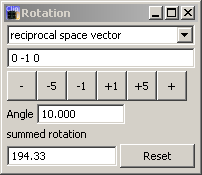
\includegraphics[width=\textwidth]{clip/Tool_Rotation}
    \label{Clip:FigToolRotation}
    \caption{Rotation tool window}
  \end{minipage}
  \imgspace{}
  \begin{minipage}[b]{0.48\textwidth}
    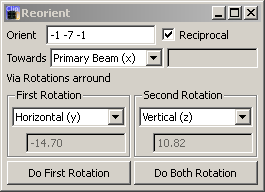
\includegraphics[width=\textwidth]{clip/Tool_Reorient}
    \label{Clip:FigToolReorient}
    \caption{Reorientation tool window}
  \end{minipage}
\end{figure}


Figure \ref{Clip:FigToolRotation} shows the rotation tool. It allows
to select one of the principal laboratory frame axes (primary beam,
horizontal or vertical) or to specify an arbitrary axis in the
laboratory frame, the reciprocal space or the direct space.
As long as the rotation axis is not changed, the rotations done around
it are summed up. Additionally provides separate buttons to quickly rotate through $\pm
1^\circ$, $\pm 5^\circ$ or $\pm$ a user defined value.

\subsection{Reorientation}

The reorientation tool \ref{Clip:FigToolReorient} allows to calculate the angles, which are
necessary to transfer the actual orientation to the desired on and
also to apply the rotations. In the top input box, the real or
reciprocal lattice vector is defined, which should be rotated towards
the direction specified in the second line. Here, the three principal
laboratory axis and arbitrary real and reciprocal lattice vectors are
possible. The lower part of the window allows to define the
goniometer axis, around which the rotations will be done.

\subsubsection{Algorithm}

To reorient two unit vectors, say \textbf{v$_1$} to \textbf{v$_2$} with two
rotations around the $\mathbf{\phi}$ and $\mathbf{\mathbf{\chi}}$ unit vectors,
\clip uses the following approach.

We we need to determine two rotation matrices $R_\phi$ and $R_\chi$, so that
$v_2 = R_\mathbf{\phi} \cdot R_\mathbf{\chi} \cdot v_1$, or equivalently
$R_\mathbf{\phi}^{-1} \cdot v_2 =  R_\mathbf{\chi} \cdot v_1$.
$R_\mathbf{\phi}^{-1} \cdot v_2$ and $R_\mathbf{\chi} \cdot v_1$ lie on a
circle on the unit sphere. These circles are the intersections of the unit
sphere with planes having $\phi$ and $\chi$ as normals and distances from the
origin of $v_2\cdot\phi$ and $v_1\cdot\chi$ respectively. These equations of
these planes are: $\mathbf{x}\cdot\mathbf{\phi}=v_2\cdot\mathbf{\phi}$ and
$\mathbf{x}\cdot\mathbf{\chi}=v_1\cdot\mathbf{\chi}$. The intersection of these
two planes is a line and the vectors on this line with a length of 1 represent
the possible intermediate vectors for the rotation: $v_i=R_\mathbf{\phi}^{-1}
\cdot \mathbf{v_2}$.

The equation of the line is
\begin{equation}
    u_1+\varepsilon\cdot u_2
    \label{lineEqn}
\end{equation}
where $u_2$ could be chosen to be perpendicular to $\mathbf{\phi}$ and
$\mathbf{\chi}$ and therefore to  be simply
$u_2=\mathbf{\phi}\times\mathbf{\chi}$ and $u_1$ could be chosen to lie in the
$\mathbf{\phi}\,\mathbf{\chi}$-plane. This gives $u_1=\lambda \cdot \phi + \mu
\cdot \chi$. The length of $u_1$ is the minimal distance of the line from the
origin and therefore determines the number of solutions. If it is larger than
one, the intersection of the two planes lie entirely outside of the unit sphere
and no rotation around $\phi$ and $\chi$ from $v_1$ to $v_2$ is possible. If
the length is exactly one, then there is one solution and corresponding one
possible rotation. If the length is smaller than one, are two possible
solutions.

To determine the coefficients in the representation of $u_1$ we consider the
equations for the two planes (remember that $u_2$ is perpendicular to both
$\chi$ and $\phi$ and therefore the product vanishes). Here we get the
equations  $(\lambda \cdot \phi + \mu \cdot \chi) \cdot \phi =
v_2\cdot\mathbf{\phi}$ and $(\lambda \cdot \phi + \mu \cdot \chi) \cdot \chi =
v_1\cdot\mathbf{\chi}$. The first equation simplifies to $\lambda  = (v_2-\mu
\cdot \chi) \cdot\mathbf{\phi}$ and inserted in the second gives the solutions

\begin{equation}
    \lambda =
    \frac{v_2\cdot\phi-(\phi\cdot\chi)(v_1\cdot\chi)}{1-(\phi\cdot\chi)^2}
\end{equation}

\begin{equation}
    \mu =
    \frac{v_1\cdot\chi-(\phi\cdot\chi)(v_2\cdot\phi)}{1-(\phi\cdot\chi)^2}
\end{equation}

If we now normalize $u_2$, we could rewrite equation (\ref{lineEqn}) as
$\varepsilon=\pm\sqrt{1-|u_1|^2}$



\subsection{Reflex Information}

The reflex info tool \ref{Clip:FigToolReflexInfo} shows the angles
between a reflex and the x-, y- and z-axis. If is in scattering
position, that is the angle to the primary beam is less than
\unit[90]{$^\circ$}, it shows Q in \AA$^{-1}$, the interplane distance d
in \AA\, and the scattering angle in $^\circ$.
The reflex could be either entered manually or clicked with an
activated info mode in the Laue Plane.


\begin{figure}[htb]
  \centering
  \begin{minipage}[b]{0.4\textwidth}
    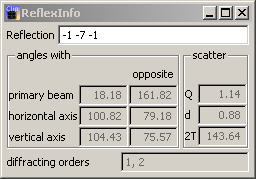
\includegraphics[width=\textwidth]{clip/Tool_ReflexInfo}
    \label{Clip:FigToolReflexInfo}
    \caption{Reflex information window}
  \end{minipage}
  \imgspace{}
  \begin{minipage}[b]{0.4\textwidth}
    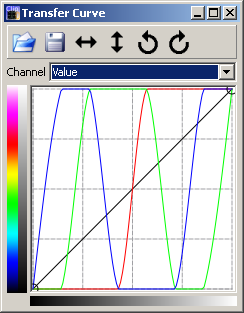
\includegraphics[width=\textwidth]{clip/Tool_TransferCurve}
    \label{Clip:FigToolTransferCurve}
    \caption{Transfer curve tool window}
  \end{minipage}
\end{figure}

\subsection{Transfer Curve}

\label{Clip:SecTransferCurve}

The image transfer curve \ref{Clip:FigToolTransferCurve} allows to
adjust the contrast of an image. It works like the corresponding tools
in various graphics softwares, like The Gimp or Adobe Photoshop.
Curves could be edited, and saved to or loaded from disk. Additionally
the image might be rotated in \unit[90]{$^\circ$} steps or flipped
horizontally or vertically. In contrast to the similar function of the
projector window, only the image itself is affected, neither the
aspect ratio not the marked spots are updated. This serves for the
case, where the image orientation is changed and afterwards spots are
marked and indexed. If know the workspace is saved and later loaded,
the spot positions does not match these of the image. Here, only (!)
the image has to be transformed. As this behavior is somewhat special,
it will be reimplemented in future versions.


\section{Future developments}


All required features for a successful treatment of Laue exposures are
basically available in Clip and the user interface is quite self
consistent. Therefore only a few features are scheduled in the short
term. These include the handling of systematic extinctions from the
space-group, the possibility to display some crystal informations on
the projection plane, an improved marker handling and performance
improvements. 

Once a marker is placed on the projector plane, the user has no chance
to tell, which marker belongs to which score, e.g. in the indexing
tool. Thus, it would be very helpful to select in the indexing window
a marker line with a bad score and get a get the corresponding marker
highlighted.

The crystal informations would include lattice
constants, orientation and some user defined text such as sample
description/identification and are most useful on printing as a
documentation. Up to now, users manually write these data on the
hardcopy. 

Long term developments depend strongly on required features. Some
possible enhancements are outlined below.

As multicore processors are more and more common, certainly more parts
of the code will ported to multithreading algorithms which in turn
would greatly improve performance.  More image processing features
could implemented, like cropping the image, background reduction or
new image formats.  Up to now, no handling of twinned crystals is
possible. It would be nice, if the twinning law could be entered to
clip and spots for different twins are marked e.g. by different
colors.

The indexing routine might be updated. Indexing relies on marking at
least two low indexed reflexes. The algorithm itself allows to use
direct space vectors instead of reciprocal space ones as input. This
would result in marking direct space vectors, or equivalently zones in
the reciprocal space. As the low index zones are clearly visible as
curved lines of bright spots, normally with clear envelope, this might
give better results in pathological cases. In fact the second edition
of clip uses this approach but it was abandoned as selecting spots
separately for indexing and refining decelerates the workflow.

Another improvement in indexing would be a fully automatic algorithm,
at least for simple problems. Wenk \etal \cite{Wenk96} propose an
algorithm where the Laue image is transformed by a gnomonic
projection. This projection transfers great circles viz. zones to
straight lines. Low indexed zones with lots of bright spots appear as
pronounced lines, which in turn are detected by a subsequent Hough
transform and a peak search algorithm. First test showed indeed human
visible straight lines, but the background of the image plate images
prevents a reliable recognition by the computer.

A model of the crystal structure could be used to calculate the 
spot intensities. This would allow to handle weak reflexes which might
not be visible on the exposure. They might just be masked if below a
certain threshold or the size of the calculated spots could scale with
calculated intensity.

At the very end, clip might support the integration of spots, scaling
them according to the wavelength distribution etc. and output in a
form suitable for single crystal refinement.



\section{Summary}

Clip has proven to be a very useful and hopefully userfriendly
program. The development basically followed the suggestions and needs
of the users \footnote{and the authors interests}, therefore some
simple features like systematic extinctions are not yet available,
while others like printing are. 

Clip has been extensively used in the institute of physics II for
orientation and checking of a whole bunch of crystals. It's algorithm
showed good performance in automatically determine the orientation for
most of the samples.

The fit procedure allows to distinguish between critical cases, if one
adopts some common crystallographic sense. The pseudo-cubic
perovskites may here serve as an example. They often crystallizes in
the orthorhombic space-group Pbnm, which emerges from the cubic base
structure by a rotation of \unit[45]{$^\circ$} around the c-axis and
doubling of the unit cell in c-direction. Thus, the lattice constants
in terms of the cubic ones a are roughly $\sqrt{2}$a, $\sqrt{2}$a, and
2a, especially with a small difference between the a and b lattice
constants. If one records a Laue pattern with the \hkl(001) in
direction of the primary beam, marks some reflexes and let the a and b
constants run during the refinement, one of them gets larger. This
allows to distinguish between the short and long in-plane axis and
works surprisingly well, even for small orthorhombic splittings.
There is one catch one should be aware of.  The long and short axis
might be reversed compared to the literature Pbnm data which
corresponds to a description in the Pnam space-group or equivalently a
renaming of a to b and vice versa. Then, if the \hkl(001) is located
near the center, the (literature) a axis lies in the direction of all \hkl(0kl)
reflexes, not \hkl(h0l) as in the case where long and short axis match
between clip and the literature.

Clip might not be finished yet, but most features for normal work use
are present. 

 



%%% Local Variables:
%%% TeX-master: "../diss"
%%% End:
